%% chapter 3

\chapter{实验设计}

\section{小鼠垂体单细胞测序}
  在小鼠垂体单细胞中进行转录组测序,然后在垂体细胞中定义和分类特定的细胞类型。
\subsection{假设}
  垂体是下丘脑的重要输出靶,并且是许多生理功能(例如生长,繁殖和内分泌释放)的中央调节器。鉴于我们了解其在释放几种主要激素中的作用,垂体细胞,特别是位于垂体前叶的垂体细胞(腺垂体)可分为五种细胞类型。

  考虑到日益发展的单细胞测序技术,可以并行分析数百个细胞,从而提供了种群中单个细胞异质性的无偏见。单细胞测序方法有很多,例如STRT(单细胞标记逆转录),CEL-seq(通过线性扩增和测序的细胞表达),Smart-seq,Smart-seq2,这些技术为我们提供了强大的工具投资很多生物学问题。尽管由于金钱和时间的浪费,这些方法只能对少量的单个细胞进行测序,但我们无法获得大型的样品库。虽然Drop-seq是一种通过将细胞包裹在微小液滴中来分析数千个单个细胞中mRNA表达的方法,但液滴-通过在微流体装置中精确结合水流和油流形成的纳升级水室已被用作PCR的微小反应室和逆转录。这种方法似乎具有很多优点,例如便宜,高效,文库质量不高,基因检测率不高等,例如每个细胞只能检测2000-3000个基因。对我们而言,重要的是选择一种基于高通量和高度自动化的适当单细胞测序方法,以确保我们可以获得高灵敏度和准确性的测序数据。

  我们从Tang Lab(FuChou Tang博士)那里获得了一种新的改进的Smart-seq2方法,该方法可最大程度地减少操作并利用单管反应来避免部分材料损失。反转录时,它将为每个细胞提供特定的细胞条形码,除了为每个mRNA提供不同的独特分子标识符(UMI)外,我们还可以将细胞集中在一起以进行测序文库构建,并使用UMI进行质量控制,以便获得高质量的单细胞基因表达数据。
\subsection{研究方法与技术路线}
\paragraph{垂体细胞解剖和消化方法的研究}
  尽管看似微不足道,但快速高效地捕获单个细胞却是单细胞测序的主要挑战之一。由于没有用于单细胞消化的标准方法,因此我们需要开发一种用于获取垂体细胞的有效方案。垂体位于下丘脑下方的颅骨底部。通过举起小鼠大脑,垂体很容易暴露,并可以直接收获结构。用无菌手术刀将腺切成小块,然后将小组织片在室温下分别在1mg / mL胶原酶\romannumeral2 和\romannumeral4 中孵育22分钟,并在消化期间上下吸移。胶原酶孵育后,在消化管中加入等体积的0.25%胰蛋白酶2分钟。消化一段时间后,我们可以使用40um过滤器收集单个细胞,然后添加相同体积的DPBS。然后将细胞悬液以1000g离心5分钟。离心后,我们丢弃上清液并将细胞重悬于DMEM培养基中。我们可以使用显微镜观察细胞状态并计数细胞数量(图\ref{fig:scseq-micro})。
\begin{figure}[!htb]
  \centering
  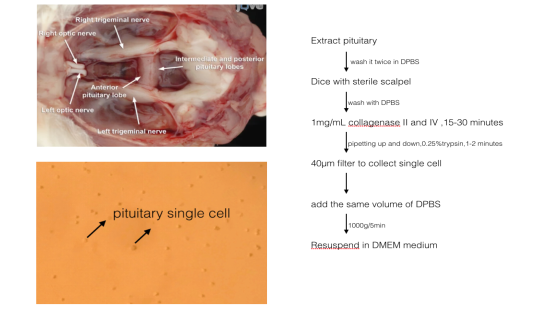
\includegraphics[width=0.8\textwidth]{figs/scseq-micro.png}
  \caption{垂体细胞解剖和消化}
  \label{fig:scseq-micro}
\end{figure}
\paragraph{使用基于smart-seq2测序的单细胞转录组分析方法获得垂体单细胞转录组}
  我们使用了改良的Smart-seq2协议,该协议是从Tang Lab获得的应用于单细胞RNA-seq的协议。简短地,垂体消化后,用白蛋白牛血清(BSA)溶液洗涤单个垂体细胞,然后通过移液管将其置于裂解缓冲液中。在逆转录反应之前,将细胞剧烈涡旋40秒,以完全裂解细胞。逆转录反应使用25 nt oligo(dT)引物进行锚定,该引物锚定有8 nt细胞特异性条形码和8 nt唯一分子标识符(UMI)。第一链合成后,合成第二链cDNA,并通过16个PCR循环扩增cDNA。然后将单个细胞的扩增cDNA汇集在一起​​以进行以下步骤。使用生物素化的预索引引物,通过另外4个PCR循环进一步扩增PCR产物,以将生物素标签引入扩增的cDNA的3'末端。 Covaris S2将大约300 ng cDNA剪切至大约300 bp,并通过Dynabeads MyOne链霉亲和素C1珠(Thermo Fisher)捕获cDNA的3'末端。 RNA-seq文库使用Kapa Hyper Prep试剂盒(Kapa Biosystems)构建,并在Illumina HiSeq 4000平台(由Novogene测序)上进行150 bp的末端测序(图\ref{fig:scseq-smart})。
\begin{figure}[!htb]
  \centering
  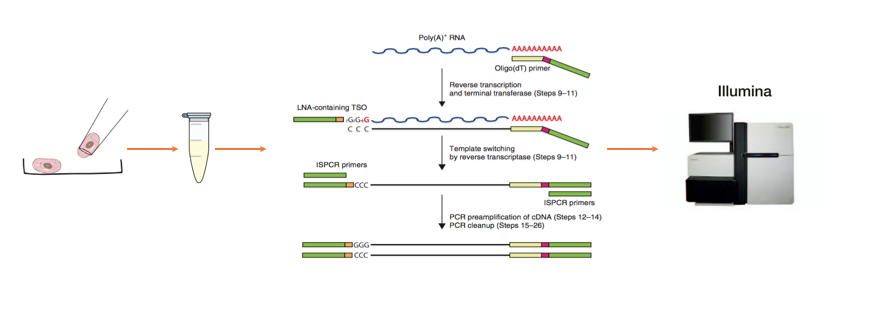
\includegraphics[width=0.8\textwidth]{figs/scseq-smart.png}
  \caption{SMART-seq2 工作流程}
  \label{fig:scseq-smart}
\end{figure}
\paragraph{单细胞测序数据分析}
  原始读段将首先被附加在双端读段的读段2中的特定细胞条形码信息分隔。将UMI信息与相应的读取1对齐,然后对其进行修剪以除去模板开关寡核苷酸(TSO)序列和poly A尾序列。随后,去除带有接头污染物和低质量碱基的读数(N>10\%)。 G1周期以外的单元也将被删除。接下来,使用TopHat(2.0.12版)将干净的读数与mm10/GRCm38对齐。然后,使用HTSeq包中的htseq-count对唯一映射的读数进行计数,并按特定于细胞的条形码分组。根据UMI信息,删除每个基因具有相同UMI序列的重复转录本。最后,将给定细胞内每个基因的不同UMI计为该基因的转录本拷贝数。对于最终的测序数据,我们将量化每个细胞中基因和转录本的数量。检测到的基因少于2000个或转录本少于100,000个的细胞将被过滤掉。表达水平通过$log_{2}(TPM/10+1)$进行归一化,其中TPM(每百万转录本)的计算方法是:每个基因的UMI数除以给定细胞的所有UMI。

  Seurat方法将用于分析关于$log_{2}(TPM/10+1)$表达值的单细胞数据。我们将使用t-SNE(t分布随机邻居嵌入)对收集单元进行分离和分类。我们将使用垂体细胞标记物来验证已测序的单个细胞实际上是来自垂体。

\subsection{可行性分析及潜在问题讨论}
  我们期望描绘小鼠垂体细胞的基因表达情况,并定义垂体中特定的细胞类型。

  因为在许多转录本测序案例中,尤其是对于单细胞测序,细胞消化可能非常具有挑战性,因为用胰蛋白酶或胶原酶对组织进行酶处理可能会对细胞活力产生未知影响,从而可能影响每个细胞的转录谱。因此,我们首先要关注的是常规的全细胞消化程序是否会人为地引起线粒体应激和转录干扰。为了解决这个问题,我们首先可以通过台盼蓝排斥试验来测试消化细胞的活力。锥虫蓝排除测试基于以下原理:活细胞具有完整的细胞膜,不包含某些染料,例如锥虫蓝,曙红或丙啶,而死细胞则没有。因此,在细胞解离后,垂体单个细胞将悬浮在含锥虫蓝的PBS中,然后进行检查以确定具有透明细胞质的细胞(活细胞)相对于具有蓝色细胞质的细胞(非活细胞)的百分比。这样,我们可以确保要测序的细胞是健康的和存活的。我们还可以通过在细胞消化过程中使用转录抑制剂(例如放线菌素D(ActD))来最大程度地减少人为诱导的转录干扰,并忠实检测基线转录谱和急性转录变化。ActD抑制所有三种真核RNA聚合酶介导的转录过程,并提供广谱,快速的转录抑制作用,几乎没有可逆的可逆性。

  该实验的主要挑战是通过手工收集可获取的垂体细胞数量有限,以及通过手工收集垂体细胞引起的潜在偏倚。细胞捕获非常耗时,并且获取足够的细胞用于细胞类型分类将花费大量的精力。除此之外,由于我们只是一厢情愿地选择完整且丰满的细胞更适合测序,因此我们会选择单个细胞,因此我们可能会错过许多看起来不如完整细胞的细胞。为了解决这个问题,我们可以将我们的原始数据与垂体发育论文上的先前论文进行比较,并更仔细地分析我们的测序数据,试图找到与300个垂体单细胞的基因相关性。我们还将尝试获取尽可能多的单个单元格以扩大样本量。

\section{建立炎症小鼠模型}
  建立病毒或细菌感染的炎症小鼠模型,并检查该炎症小鼠模型的可行性。
\subsection{假设}
  垂体在调节人体的生长,发育及许多其他重要功能中起着关键作用,它是HPA轴的一部分,并且是大脑的内分泌中心,它控制激素的分泌。炎性细胞因子可以刺激垂体释放激素的分泌,例如肾上腺皮质激素和β-内啡肽,它们对炎症或应激刺激具有抗炎特性。垂体前叶细胞可产生IL1和IL6,这可能会影响局部激素的产生。因此,垂体积极参与免疫反应和炎症过程。

  LPS和Poly I:C在炎症过程中是有效的免疫刺激。它们的行为就像细菌或病毒感染一样。将此类免疫激活剂应用于小鼠可引起严重的免疫反应。我们建议使用行为范式和细胞因子Elisa方法来测试使用LPS和Poly I:C诱导炎性小鼠模型的可行性。使用可靠的炎症反应小鼠模型,可以轻松地进行进一步的测序实验,以测试炎症诱导的小鼠垂体细胞转录谱的变化。
\subsection{研究方法与技术路线}
\paragraph{给小鼠外周注射LPS或Poly I:C以模仿细菌或病毒感染,或外周注射TNF-$\alpha$模仿炎症反应}
  由于垂体内分泌细胞与激素分泌有关,而垂体细胞可能受到雌性激素水平的影响,因此我们选择只使用雄性小鼠进行实验,以保证实验数据的一致性。我们将分析急性LPS和细胞因子刺激后的免疫反应。

  将两个月大的小鼠随机分配至治疗组,并以每公斤体重50 mg的剂量通过细菌性脂多糖(来自大肠杆菌O111:B4,Sigma的LPS)进行腹膜内(ip)注射,并使用双链RNA Polyinosinic–聚胞苷酸钠盐(Sigma公司生产的Poly I:C),每公斤体重20mg。对于外周细胞因子治疗,将以重组小鼠细胞因子TNF-α处理小鼠,剂量为每公斤体重500μg。用于对照实验的小鼠将接受媒介物注射(盐水)。注射药物后,等待约6个小时,对小鼠进行开放式试验,并从眼眶中收集全血。
\paragraph{通过行为测试范例测试炎性小鼠模型的可行性}
  免疫刺激注射已显示出诱导免疫攻击和疾病行为,运动能力的持续下降表明。我们使用开放式试验中运动的减少作为检验炎症诱导小鼠模型的功效和可行性的基准。

  免疫刺激约6小时后,将对小鼠进行公开测试。野外测试使用一个大的立方体箱,长1m×宽1m×高1m。立方体的顶部通常不被覆盖。我们将鼠标放在底部表面的中间,随着鼠标自由移动并探索环境,在5分钟的过程中记录了鼠标的移动。在测试过程中,我们将通过相机记录其运动轨迹。测试完成后,将使用计算机跟踪程序(MATLAB)分析动物随时间的运动。在野外试验之后,我们将比较炎症诱发小鼠和对照小鼠之间的运动,以得出有关炎症诱发小鼠模型可行性的结论。
\paragraph{测量血液促炎细胞因子水平}
  对我们而言,收集小鼠炎症信息很重要。 免疫刺激约6小时后,我们将通过Elisa试剂盒从眼眶收集全血并测量血液促炎细胞因子,例如IL-1,IL-6,TNF-$\alpha$。 同时,将通过定量PCR评估垂体解剖中TNF-$\alpha$,IL-1,IL-6的mRNA水平。

\subsection{可行性分析及潜在问题讨论}
  在可行的炎症诱导的小鼠模型中,我们期望看到减少的运动,通过Elisa血液样本测定的促炎因子水平升高以及通过qPCR评估的垂体细胞促炎因子mRNA水平升高。这些指标在治疗(注射Poly I:C,LPS,TNF-$\alpha$)与对照组之间的小鼠重复测量中应保持一致,这将有助于我们得出结论:炎症诱导的小鼠模型是可行的。

  该实验的主要挑战将是Poly I:C注射是否会导致对小鼠的一致性免疫作用。在我们的一些初步测试中,我们发现即使高剂量的Poly I:C注射后,一部分小鼠仍对Poly I:C表现出极大的抵抗力。这些小鼠保持活跃,垂体细胞转录组的测序数据与对照小鼠一样正常。这使我们相信,在进行以下实验之前,必须进行行为测试和细胞因子测试。根据我们的协议,如果在行为测试和血液细胞因子测试中,鼠标碰巧显示出对Poly I:C注射的抗性,我们将不会对鼠标执行单细胞测序。

  我们将尝试找到一种更稳定的方法来建立病毒/细菌感染的小鼠模型。

\section{验证炎症条件下生物标志物}
  剖析垂体功能性单细胞命运的变化,并验证炎症条件下分泌激素的功能以及生物标志物。
\subsection{假设}
  单细胞RNA测序技术的快速发展为我们提供了高效的工作流程,即使我们以前的基因知识有限或猜测工作繁重,也使我们能够获取单个细胞的转录信息。这项技术已在科学研究的各个方面使用。例如,在开发领域,它扩展了我们在个体开发过程中的知识,并帮助我们识别了未知的细胞标志物和多种细胞类型。在癌症领域,这项技术已帮助我们识别癌症类型,并帮助进行特定的医学诊断和个性化治疗。

  单细胞RNA测序技术对免疫研究也有很大影响。例如,最近,对免疫细胞的研究表明,即使是从看似均一的种群中衍生出来的,单个细胞在其基因表达,蛋白质水平或表型输出方面也可能表现出对外部刺激的不同反应。麻省理工学院和哈佛大学的研究小组使用单细胞RNA测序方法发现,LPS处理后,骨髓来源的树突状细胞(BMDC)在每个细胞中的基因表达和剪接模式都有很大的差异。显然,单小区技术可用于发现小区与小区网络之间的各种功能或响应。这些对健康和疾病组织的初步研究为我们进一步研究免疫刺激反应的单个细胞功能铺平了道路。

  在这里,我们将使用免疫刺激来研究炎症激发是否会导致参与免疫应答的垂体细胞转录的改变。我们将使用不同剂量的相同免疫刺激,并将免疫刺激在不同时间点应用于小鼠。根据我们的初步数据,我们想知道当垂体单细胞受到免疫刺激时是否存在命运改变点。我们相信,每种炎症都有一个独特的生物标志物,经过仔细的数据分析,可以得到用于免疫诊断的标志物。在此过程中,我们将尝试基于单细胞转录组测序分析寻找垂体中未知的分泌激素,并通过RNA原位杂交或免疫染色找出激素的靶向脑区域。
\subsection{研究方法与技术路线}
\paragraph{给小鼠外周注射高剂量或低剂量的LPS,在不同时间点应用刺激剂,以探索细菌对小鼠的影响}
  我们仅使用雄性小鼠来保证实验数据的一致性,并避免雌性激素引起的可能干扰。将两个月大的小鼠随机分配至治疗组,并以每公斤体重50 mg(高剂量)和每公斤体重10 mg(低剂量)的剂量腹膜内(i.p.)注射LPS。对于每剂LPS,我们将采用两种不同的时间范围,一种是6小时(急性反应较长时间),另一种是3小时(急性反应较短时间)。免疫刺激后,将对小鼠进行野外试验,并从眼眶中收集全血。垂体细胞的单细胞测序将随后进行。我们将通过解剖提取垂体小鼠,并将细胞消化成单细胞悬液。然后,我们将使用基于smart-seq2测序的单细胞转录组分析方法来获得响应LPS给药的垂体单细胞转录谱,并分析剂量和时间尺度对垂体细胞的影响。
\paragraph{给小鼠外周注射高剂量或低剂量的Poly I:C,在不同的时间应用刺激,以探索病毒对小鼠的影响}
  如上所述,我们仅使用雄性小鼠进行实验。 将两个月大的小鼠随机分配至治疗组,并以20 mg / kg体重(高剂量)和10mg / kg体重(低剂量)的剂量腹膜内(ip)注射poly I:C。 Poly I:C的剂量我们将使用两种不同的时间尺度,一种是6小时(急性反应较长时间),另一种是3小时(急性反应较短时间)。在免疫刺激后,对小鼠进行免疫 进行野外测试,并从轨道收集全血。 垂体细胞的单细胞测序将随后进行。 我们将使用smart-seq2获得响应poly I:C给药的垂体单细胞转录谱,并分析剂量和时间尺度对垂体细胞的影响。
\paragraph{给小鼠外周注射高剂量或低剂量的TNF-$\alpha$,以探讨促炎作用对小鼠的影响}
  我们使用雄性小鼠进行实验。 将两个月大的小鼠随机分配至治疗组,并以每千克体重500μg的剂量腹膜内(ip)注射促炎性TNF-$\alpha$(小鼠,Sigma),并等待6小时和1 mg / kg 体重,等待6小时。 注射免疫刺激后,我们测试小鼠的运动能力并从眼眶中提取全血以进行垂体单细胞RNA测序。 我们将使用smart-seq2获得对高剂量或低剂量TNF-$\alpha$响应的垂体细胞的转录谱(图\ref{fig:scseq-expr})。
\begin{figure}[!htb]
  \centering
  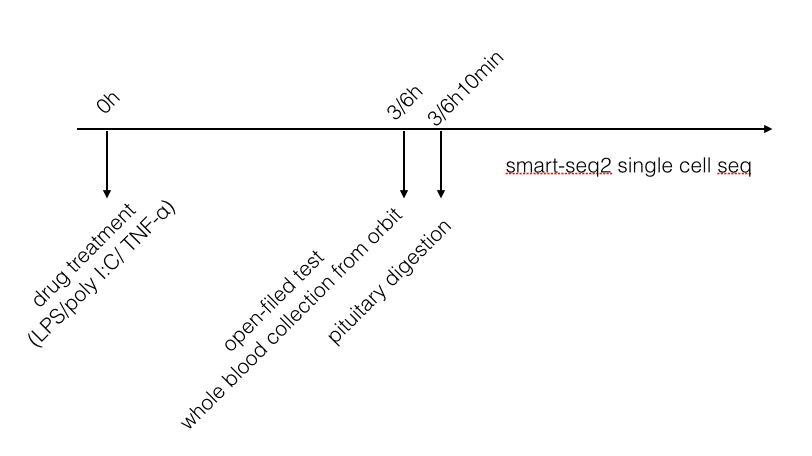
\includegraphics[width=0.8\textwidth]{figs/scseq-expr.png}
  \caption{实验工作流程}
  \label{fig:scseq-expr}
\end{figure}

\paragraph{对四种药物治疗的转录谱进行数据分析}
  根据测序结果,我们将使用t-SNE(t分布随机邻居嵌入)对我们收集的转录谱进行分组和分类,并使用垂体细胞标记物验证测序数据。 将制作细胞谱图,以找出炎症治疗与基因表达谱之间的关系。 如果我们能够在不同的免疫挑战条件和不同的免疫刺激时间尺度下鉴定出特定的炎症生物标记,那将是理想的。
\paragraph{通过原位杂交,细胞因子Elisa或Western blot验证炎症测序结果}
  收集数据后,我们将使用RT PCR或原位杂交来验证测序数据。 如果观察到未知的分泌激素,我们将尝试通过免疫染色鉴定其靶标大脑区域或通过体外筛选测定法找到其靶标受体。

\subsection{可行性分析及潜在问题讨论}
  我们期望观察在不同的免疫挑战条件下获得的特异性生物标志物。 但是,主要问题是数据批处理效果和数据质量。因为我们使用移液器收集单个细胞,所以收集到的细胞可能会有偏差。 而且,由于长的细胞采摘时间,细胞活力将被削弱。不同的人和不同的操作时间将导致对细胞的未知影响。为了降低主观效果,将需要对细胞分类进行更多的实践以缩短拣选时间,并且必须优化细胞拣选工作流程。我们还将每次都准备更多的细胞库以降低批次效应。

